\documentclass[11pt,a4paper]{article}

% --- Packages fondamentaux ---
\usepackage[utf8]{inputenc}
\usepackage[T1]{fontenc}
\usepackage[french]{babel}
\usepackage{geometry}
\geometry{top=2.5cm, bottom=2.5cm, left=2.2cm, right=2.2cm, headheight=15pt}

\usepackage{xcolor}
\usepackage{colortbl}
\usepackage{graphicx}
\usepackage{hyperref}
\usepackage{amsmath,amssymb}
\usepackage{booktabs}
\usepackage{tabularx}
\usepackage{array}
\usepackage{fancyhdr}
\usepackage{listings}
\usepackage{enumitem}
\usepackage{tcolorbox}
\tcbuselibrary{skins,breakable}

% --- Palette de couleurs NOVA ---
\definecolor{novabg}{HTML}{080A10}
\definecolor{novasurface}{HTML}{11141C}
\definecolor{novasurface2}{HTML}{171A24}
\definecolor{novapurple}{HTML}{8B5CF6}
\definecolor{novapurpledark}{HTML}{6D28D9}
\definecolor{novagreen}{HTML}{22C55E}
\definecolor{novared}{HTML}{EF4444}
\definecolor{novaamber}{HTML}{F59E0B}
\definecolor{novagray}{HTML}{4B5563}
\definecolor{novalightgray}{HTML}{9CA3AF}

% --- Configuration Hyperref ---
\hypersetup{
    colorlinks=true,
    linkcolor=novapurpledark,
    citecolor=novapurpledark,
    urlcolor=novapurple,
    pdfauthor={Equipe Architecture et Securite NOVA},
    pdftitle={NOVA Chat - Dossier d'Architecture Technique, Securite et Multiplateforme},
    pdfsubject={Messagerie P2P Souveraine et Décentralisée},
    pdfkeywords={P2P, QUIC, Rust, Flutter, Double Ratchet, E2EE, Securite, Multiplateforme}
}

% --- Configuration Listings ---
\lstset{
    basicstyle=\ttfamily\small,
    backgroundcolor=\color{novasurface2!10},
    keywordstyle=\color{novapurpledark}\bfseries,
    stringstyle=\color{novagreen!80!black},
    commentstyle=\color{novalightgray}\itshape,
    numbers=left,
    numberstyle=\tiny\color{novagray},
    numbersep=8pt,
    frame=single,
    rulecolor=\color{novapurple!30},
    breaklines=true,
    showstringspaces=false,
    tabsize=2
}

% --- Boîtes personnalisées ---
\newtcolorbox{infobox}[1][]{
    enhanced,
    colback=novasurface2!5,
    colframe=novapurple,
    arc=4mm,
    boxrule=1.2pt,
    left=12pt, right=12pt, top=10pt, bottom=10pt,
    title=#1,
    coltitle=white,
    fonttitle=\bfseries\color{white},
    attach boxed title to top left={yshift=-2mm, xshift=4mm},
    boxed title style={colback=novapurpledark, arc=2mm, boxrule=0pt}
}

\newtcolorbox{securitybox}[1][]{
    enhanced,
    colback=novared!5,
    colframe=novared,
    arc=4mm,
    boxrule=1.2pt,
    left=12pt, right=12pt, top=10pt, bottom=10pt,
    title=#1,
    coltitle=white,
    fonttitle=\bfseries\color{white},
    attach boxed title to top left={yshift=-2mm, xshift=4mm},
    boxed title style={colback=novared!80!black, arc=2mm, boxrule=0pt}
}

% --- En-têtes et pieds de page ---
\pagestyle{fancy}
\fancyhf{}
\lhead{\textcolor{novagray}{\small\textbf{NOVA Chat} — Architecture \& Spécifications Techniques}}
\rhead{\textcolor{novagray}{\small Version 1.0}}
\cfoot{\textcolor{novagray}{\small Page \thepage}}
\renewcommand{\headrulewidth}{0.4pt}
\renewcommand{\footrulewidth}{0.4pt}

\begin{document}

% =========================================================================
% PAGE DE GARDE
% =========================================================================
\begin{titlepage}
    \pagecolor{novabg}
    \color{white}
    \begin{center}
        \vspace*{1.5cm}
        
        {\Huge \textbf{\textcolor{novapurple}{NOVA CHAT}}}\\[0.4cm]
        {\Large \textbf{Système de Messagerie Souveraine P2P Décentralisée}}\\[0.2cm]
        {\large \textcolor{novalightgray}{Architecture Système, Modèle Cryptographique, Multiplateforme \& Staffing}}
        
        \vspace{1.2cm}
        \rule{0.8\textwidth}{1.5pt}
        \vspace{1.2cm}
        
        \begin{tcolorbox}[
            enhanced,
            colback=novasurface,
            colframe=novapurple,
            arc=5mm,
            width=0.9\textwidth,
            boxrule=1.5pt,
            center
        ]
            \centering
            \vspace{0.3cm}
            {\large \textbf{\textcolor{white}{DOSSIER D'INGÉNIERIE \& D'ARCHITECTURE LOGICIELLE}}}\\[0.3cm]
            \textcolor{novalightgray}{
                \textbf{Cibles :} Mobile (Android, iOS) $\bullet$ Tablette (iPadOS, Android) $\bullet$ PC (Windows, macOS, Linux)\\[0.15cm]
                \textbf{Noyau :} Rust Core (QUIC, X3DH, Double Ratchet, SQLCipher, Hole Punching)\\[0.15cm]
                \textbf{Interface :} Flutter Multiplatform Responsive (17 Écrans Conformes)
            }
            \vspace{0.3cm}
        \end{tcolorbox}
        
        \vfill
        
        \begin{minipage}{0.45\textwidth}
            \begin{flushleft} \large
                \textbf{\textcolor{novapurple}{Auteurs :}} \\
                Équipe Architecture Logicielle \\
                Pôle Sécurité \& Cryptographie \\
                Département Réseaux P2P
            \end{flushleft}
        \end{minipage}
        \begin{minipage}{0.45\textwidth}
            \begin{flushright} \large
                \textbf{\textcolor{novapurple}{Statut :}} \\
                Version 1.0 — Validée \\
                Projet Indépendant \\
                Août 2026
            \end{flushright}
        \end{minipage}
        
        \vspace{1.0cm}
    \end{center}
\end{titlepage}

\nopagecolor
\color{black}

% =========================================================================
% TABLE DES MATIÈRES
% =========================================================================
\tableofcontents
\newpage

% =========================================================================
% 1. SYNTHÈSE EXÉCUTIVE & VISION TECHNIQUE
% =========================================================================
\section{Synthèse Exécutive \& Vision Technique}

\subsection{Objectif Fondamental : Le Paradigme de Souveraineté}
Le projet \textbf{NOVA Chat} vise à concevoir une application de messagerie moderne, hautement sécurisée et décentralisée, permettant à deux pairs ($A \leftrightarrow B$) d'échanger des messages, des fichiers et des appels directement via Internet, \textbf{sans dépendre d'un serveur cloud permanent pour transporter ou stocker les données}.

Contrairement aux architectures conventionnelles de messagerie (WhatsApp, Signal, Telegram), le serveur distant ne constitue en aucun cas un centre de stockage ou de routage obligatoire :
\begin{itemize}[leftmargin=1.5cm]
    \item \textbf{Zéro Base de Données Centrale} : Aucune trace des conversations, profils ou carnets de contacts n'existe en dehors des terminaux des utilisateurs.
    \item \textbf{Zéro Clé Privée Distante} : Les identités cryptographiques sont générées localement et ne quittent jamais l'enclave sécurisée de l'appareil.
    \item \textbf{Serveur de Découverte Éphémère} : Le serveur externe agit comme un simple facilitateur de mise en relation (\textit{Signaling / STUN}), intervenant uniquement au moment de l'établissement de la liaison.
    \item \textbf{Relais Aveugle Temporaire (\textit{Blind Relay})} : En cas d'impossibilité physique de traverser un NAT strict, un relais achemine des paquets chiffrés de bout-en-bout sans jamais pouvoir en lire le contenu ni en conserver d'historique.
\end{itemize}

\begin{infobox}[Principe Directeur]
\textbf{Le serveur aide A et B à se trouver, mais ne devient jamais le serveur de messagerie.} Chaque appareil est un nœud souverain (\textit{Peer Agent}) orchestrant sa propre cryptographie, son stockage et ses files d'attente.
\end{infobox}

\vspace{0.3cm}

% =========================================================================
% 2. ARCHITECTURE SYSTÈME & TOPOLOGIE RÉSEAU
% =========================================================================
\section{Architecture Système \& Topologie Réseau}

\subsection{Modèle en 4 Couches Étanche}
Pour garantir la maintenabilité, la portabilité multiplateforme et la sécurité, le système est structuré en quatre couches indépendantes :

\begin{center}
\begin{tabularx}{0.95\textwidth}{|c|X|}
\hline
\rowcolor{novasurface2!20} \textbf{Couche} & \textbf{Rôle et Responsabilités} \\ \hline
\textbf{1. Application \& UI} & Interface graphique réactive (Flutter), gestion d'état déclarative (MVI / BLoC), affichage transparent des statuts P2P (Direct / Relayé / Hors-ligne). \\ \hline
\textbf{2. Moteur de Messagerie} & Gestion de l'identité locale (BIP-39, Ed25519), sessions E2EE (Double Ratchet), file d'attente sortante (\textit{Outbox Engine}), base locale chiffrée (SQLCipher). \\ \hline
\textbf{3. Transport P2P} & Négociation de session QUIC/UDP, traversée NAT (\textit{STUN Hole Punching}), Keep-Alive adaptatif, routage vers le relais éphémère si requis. \\ \hline
\textbf{4. Réseau Physique} & Couche IP/UDP sous-jacente (Wi-Fi, 4G, 5G, Ethernet). \\ \hline
\end{tabularx}
\end{center}

\subsection{Stratégie de Traversée NAT (NAT Traversal)}
Le principal verrou technologique des communications P2P sur réseaux mobiles réside dans la présence de pare-feux et de routeurs avec NAT symétrique (\textit{Carrier-Grade NAT / CGNAT}). La stratégie d'établissement de liaison de NOVA suit un algorithme à trois niveaux :

\begin{enumerate}[leftmargin=1.2cm]
    \item \textbf{Niveau 1 — Connexion Directe UDP Hole Punching} : 
    Les nœuds interrogent le serveur de découverte pour déterminer leurs adresses IP/Ports réflexifs (STUN). Les deux pairs émettent simultanément des datagrammes UDP l'un vers l'autre pour ouvrir les tables de routage NAT et établir un socket direct. Taux de succès estimé : $70\text{--}85\%$.
    \item \textbf{Niveau 2 — Connexion en Réseau Local (LAN / Wi-Fi)} : 
    Si les appareils partagent le même sous-réseau, la découverte s'effectue automatiquement via mDNS / Multicast UDP sans passer par Internet.
    \item \textbf{Niveau 3 — Relais Chiffré Opaque (\textit{Zero-Knowledge Fallback})} : 
    En cas de double NAT symétrique restrictif, la communication bascule de manière transparente sur un relais éphémère. Le relais ne reçoit que des blocs chiffrés par la clé de session $A \leftrightarrow B$. Dès distribution, le paquet est purgé de la mémoire vive du relais.
\end{enumerate}

\subsection{Choix du Protocole de Transport : QUIC vs WebRTC vs TCP}
Le protocole \textbf{QUIC} (sur UDP) a été retenu au détriment de WebRTC et TCP pour les raisons techniques suivantes :
\begin{itemize}
    \item \textbf{Mobilité Réseau (\textit{Connection Migration})} : Lorsqu'un smartphone bascule de la 4G/5G vers un réseau Wi-Fi, l'adresse IP change. Grâce aux \textit{Connection IDs} de QUIC, la session de communication reste active sans rupture ni ré-authentification.
    \item \textbf{Multiplexage sans blocage de tête de ligne (\textit{Head-of-Line Blocking})} : Les messages textuels, les accusés de réception et les morceaux de fichiers volumineux sont envoyés sur des flux QUIC indépendants.
    \item \textbf{Latence Réduite} : Établissement de session en 0-RTT / 1-RTT avec chiffrement TLS 1.3 intégré au niveau transport.
\end{itemize}

\vspace{0.3cm}

% =========================================================================
% 3. CONCEPTION CRYPTOGRAPHIQUE & SÉCURITÉ FORMELLE
% =========================================================================
\section{Conception Cryptographique \& Sécurité Formelle}

\subsection{Primitives Cryptographiques de l'État de l'Art}
NOVA Chat intègre une suite cryptographique moderne, performante et formellement prouvée :

\begin{table}[h!]
\centering
\begin{tabularx}{\textwidth}{|l|l|X|}
\hline
\rowcolor{novasurface2!20} \textbf{Fonction} & \textbf{Primitive} & \textbf{Rôle dans NOVA Chat} \\ \hline
Identité \& Signature & \textbf{Ed25519} & Signature des profils, annonces de présence et messages de contrôle. \\ \hline
Échange de Clés & \textbf{X25519} & Handshake asynchrone (Diffie-Hellman) et rotation de session. \\ \hline
Chiffrement Authentifié & \textbf{ChaCha20-Poly1305} & AEAD 256 bits garantissant confidentialité et intégrité des charges utiles. \\ \hline
Hachage \& KDF & \textbf{BLAKE3 / HKDF-SHA256} & Dérivation des chaînes de clés de message et empreintes d'identité. \\ \hline
Dérivation Maîtresse & \textbf{Argon2id + BIP-39} & Génération de la clé d'identité racine à partir d'une phrase mnémonique de 12 mots. \\ \hline
\end{tabularx}
\caption{Primitives cryptographiques sélectionnées pour le moteur souverain.}
\end{table}

\subsection{Protocole Double Ratchet \& Propriétés de Sécurité}
Chaque conversation individuelle ($A \leftrightarrow B$) instancie une session gouvernée par le protocole \textbf{Double Ratchet} :
\begin{itemize}
    \item \textbf{Perfect Forward Secrecy (PFS)} : Chaque message est chiffré avec une clé éphémère unique. Dès qu'un message est déchiffré, sa clé est immédiatement détruite en mémoire (\texttt{zeroize}). La compromission ultérieure de l'appareil ne permet pas de déchiffrer le trafic passé.
    \item \textbf{Post-Compromise Security (PCS)} : Si un attaquant capture temporairement les clés de session, l'envoi d'un nouvel échange Diffie-Hellman par le correspondant légitime restaure automatiquement le secret de la session.
\end{itemize}

\subsection{Consolidation du Chiffrement 1-to-1 \& Isolation des Sessions}
Dans l'architecture souveraine NOVA Chat, chaque paire d'utilisateurs ($A \leftrightarrow B$) maintient une session cryptographique strictement isolée :
\begin{itemize}
    \item \textbf{Isolation Totale} : La compromission d'une session avec un pair $C$ n'a strictement aucun impact sur les secrets échangés avec $B$.
    \item \textbf{Clés Éphémères Uniques} : Aucune clé de session n'est partagée ou réutilisée entre différents contacts.
    \item \textbf{Validation d'Empreinte Déterministe} : Vérification hors-bande symétrique par Safety Numbers (BLAKE3) directement intégrée à chaque fiche de contact.
\end{itemize}

\subsection{Modèle de Menace \& Matrice de Risques (STRIDE)}

\begin{table}[h!]
\centering
\small
\begin{tabularx}{\textwidth}{|l|X|X|}
\hline
\rowcolor{novasurface2!20} \textbf{Menace STRIDE} & \textbf{Vecteur d'Attaque Potentiel} & \textbf{Contre-Mesure Implémentée dans NOVA} \\ \hline
\textbf{Spoofing} & Usurpation d'identité sur le serveur de découverte. & Authentification par signature Ed25519 de chaque paquet d'enregistrement. \\ \hline
\textbf{Tampering} & Altération de paquets par un routeur ou le relais. & Chiffrement AEAD ChaCha20-Poly1305 (rejet immédiat si le tag est altéré). \\ \hline
\textbf{Repudiation} & Répudiation de l'envoi d'un message. & Numérotation de séquence cryptographique et chaînage de hachage. \\ \hline
\textbf{Information Leak} & Interception du trafic et analyse de métadonnées. & Enveloppes aveugles sur le relais, TLS 1.3 sur QUIC, SQLCipher AES-256 local. \\ \hline
\textbf{Denial of Service} & Inondation du serveur de présence. & Preuve de travail (PoW) légère type Hashcash à l'inscription + Rate Limiting. \\ \hline
\textbf{Elevation} & Fichier malveillant / Pièce jointe piégée. & Isolation mémoire en Rust (Zero-Copy), sandboxing strict des pièces jointes. \\ \hline
\end{tabularx}
\caption{Matrice d'analyse des menaces STRIDE et mesures de mitigation.}
\end{table}

\vspace{0.3cm}

% =========================================================================
% 4. ANALYSE MULTIPLATEFORME & BENCHMARK TECHNOLOGIQUE
% =========================================================================
\section{Analyse Multiplateforme (PC, Tablette, Mobile) \& Choix Technologique}

\subsection{Objectif Multi-Appareil}
L'application doit s'exécuter de manière fluide sur :
\begin{itemize}
    \item \textbf{Mobile} : Smartphones Android (ARM64, ARMv7) et Apple iOS (ARM64).
    \item \textbf{Tablette} : iPadOS et Tablettes Android (mode portrait et paysage adaptatif).
    \item \textbf{PC Desktop} : Windows (x86\_64, ARM64), macOS (Apple Silicon, Intel) et Linux (x86\_64).
\end{itemize}

\subsection{Benchmark Comparatif des Stacks}

\begin{table}[h!]
\centering
\small
\begin{tabularx}{\textwidth}{|l|c|c|c|c|}
\hline
\rowcolor{novasurface2!20} \textbf{Critère d'Évaluation} & \textbf{Flutter + Rust} & \textbf{Compose MP + Rust} & \textbf{Tauri 2.0 (Web)} & \textbf{React Native} \\ \hline
Couverture des 5 plateformes & \textbf{Excellente (100\%)} & Bonne (Desktop JVM) & Excellente & Moyenne (Desktop séparé) \\ \hline
Performance UI \& Fluidité & \textbf{120 fps (Impeller)} & 60-120 fps (Skiko) & 60 fps (WebView) & 60 fps (Fabric) \\ \hline
Intégration Rust / Zero-Copy & \textbf{Directe (FRB v2)} & UniFFI / JNI & Natif (Rust Core) & JSI complexe \\ \hline
Consommation RAM Desktop & \textbf{Faible ($\sim$45 Mo)} & Haute ($\sim$180 Mo) & \textbf{Faible ($\sim$35 Mo)} & Très haute ($\sim$250 Mo) \\ \hline
Adaptabilité Tablette / PC & \textbf{Excellente} & Excellente & Bonne & Moyenne \\ \hline
Coût de développement & \textbf{Minimal (1 base)} & Moyen & Moyen & Élevé \\ \hline
\textbf{Note Globale} & \textbf{9.5 / 10} & 8.0 / 10 & 7.5 / 10 & 6.0 / 10 \\ \hline
\end{tabularx}
\caption{Comparatif technique des architectures pour NOVA Chat.}
\end{table}

\subsection{Recommandation Stratégique : Flutter + Core Rust (\texttt{flutter\_rust\_bridge})}
L'architecture validée repose sur un couplage étanche :
\begin{enumerate}
    \item \textbf{Moteur Système Unifié (Rust)} : Compile en bibliothèques natives (\texttt{.so}, \texttt{.dylib}, \texttt{.dll}, \texttt{.a}) partagées entre tous les systèmes.
    \item \textbf{Couche Graphique Déclarative (Flutter)} : Un code unique pilote l'interface utilisateur sur mobile, tablette et PC avec un rendu GPU direct (sans WebView).
\end{enumerate}

\subsection{Gestion Adaptative des Écrans (Responsive Breakpoints)}
\begin{itemize}
    \item \textbf{Mobile ($< 600\text{ dp}$)} : Vue mono-colonne. Navigation basse à 3 onglets (Conversations, Contacts, Réglages).
    \item \textbf{Tablette ($600\text{ dp} \le \text{width} < 1024\text{ dp}$)} : Vue \textit{Split-View} à 2 colonnes (Liste des conversations à gauche, zone de chat active à droite).
    \item \textbf{Desktop ($> 1024\text{ dp}$)} : Vue \textit{Triple-Pane} (Barre de navigation latérale compacte + Liste des contacts/conversations + Zone de chat active + Volet d'informations de sécurité et médias).
\end{itemize}

\vspace{0.3cm}

% =========================================================================
% 5. SYSTÈME DE DESIGN & LES 17 ÉCRANS
% =========================================================================
\section{Système de Design \& Spécification des 17 Écrans}

\subsection{Palette Visuelle \& Tokens de Design}
L'identité visuelle est résolument moderne, technologique, sombre et orientée confidentialité :

\begin{center}
\begin{tabularx}{0.95\textwidth}{|l|l|X|}
\hline
\rowcolor{novasurface2!20} \textbf{Élément} & \textbf{Code Couleur} & \textbf{Usage dans l'interface} \\ \hline
Background Principal & \texttt{\#080A10} & Fond d'écran global de l'application. \\ \hline
Surface 1 (Cartes/Éléments) & \texttt{\#11141C} & Cartes de profil, champs de recherche, bulles reçues. \\ \hline
Surface 2 (Élévation) & \texttt{\#171A24} & En-têtes, barres d'outils, conteneurs secondaires. \\ \hline
Surface Active & \texttt{\#202431} & Éléments sélectionnés, hover, bordures actives. \\ \hline
Accent Principal & \texttt{\#8B5CF6} & Boutons d'action majeurs, bulles de message émis, sécurité. \\ \hline
Indicateur Direct P2P & \texttt{\#22C55E} & Pastille de statut \textbf{\textcolor{novagreen}{$\bullet$} Direct} (connexion active). \\ \hline
Indicateur Relayé & \texttt{\#F59E0B} & Pastille de statut \textbf{\textcolor{novaamber}{$\nearrow$} Relayé} (transit chiffré temporaire). \\ \hline
Indicateur Hors-Ligne & \texttt{\#6B7280} & Pastille de statut \textbf{\textcolor{novagray}{$\circ$} Hors ligne}. \\ \hline
\end{tabularx}
\end{center}

\subsection{Aperçu de la Maquette Graphique}
La figure \ref{fig:mockup} illustre la construction graphique des écrans clés validés pour NOVA Chat :

\begin{figure}[h!]
    \centering
    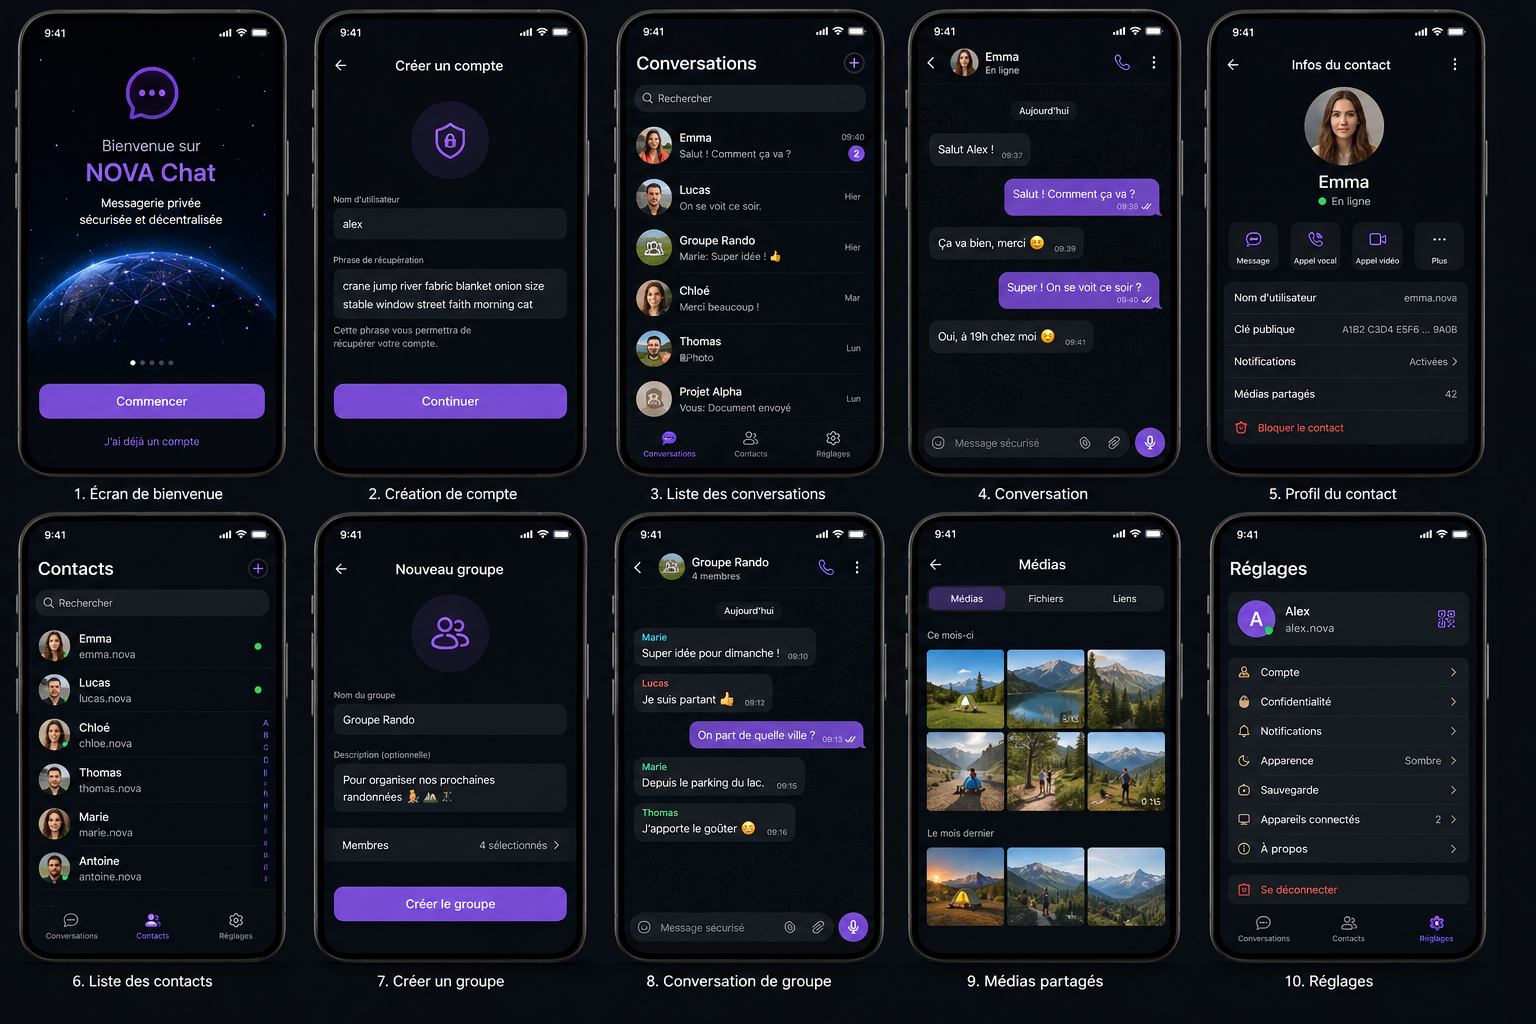
\includegraphics[width=0.98\textwidth]{mockup.png}
    \caption{Maquette d'interface NOVA Chat : Écrans de Bienvenue, Création de compte, Liste des conversations, Conversation 1-on-1, Profil de contact, Contacts, Nouveau groupe, Discussion de groupe, Médias partagés et Réglages.}
    \label{fig:mockup}
\end{figure}

\subsection{Cartographie Complète des 17 Écrans}
\begin{enumerate}
    \item \textbf{Écran 1 — Bienvenue (\texttt{/onboarding})} : Globe réseau avec nœuds interconnectés, slogan, boutons « Commencer » et « J'ai déjà un compte ».
    \item \textbf{Écran 2 — Création de compte (\texttt{/onboarding/create-account})} : Génération locale de la clé privée et affichage de la phrase mnémonique de récupération (12 mots BIP-39).
    \item \textbf{Écran 3 — Liste des conversations (\texttt{/conversations})} : Liste dynamique des discussions, badges de messages non-lus, barre de recherche et indicateurs de liaison P2P directe.
    \item \textbf{Écran 4 — Conversation individuelle (\texttt{/chat/:id})} : En-tête sécurisé avec statut P2P, bulles de messages émis (violet) / reçus (sombre), accusés d'état (\checkmark\checkmark), tiroir de pièces jointes (fichiers, photos, audio) et sélecteur de stickers.
    \item \textbf{Écran 5 — Profil du contact (\texttt{/contact/:id})} : Avatar, nom d'utilisateur (\texttt{emma.nova}), clé publique tronquée, actions rapides (Message, Appel vocal, Vidéo), Safety Number et option de blocage.
    \item \textbf{Écran 6 — Liste des contacts (\texttt{/contacts})} : Annuaire local des pairs avec indexation alphabétique, indicateur de présence instantanée et bouton d'ajout.
    \item \textbf{Écran 7 — Ajouter un contact (\texttt{/contacts/add})} : Recherche par nom d'utilisateur, scanner de QR Code d'identité et affichage de son propre QR Code public.
    \item \textbf{Écran 8 — Créer un groupe (\texttt{/groups/create})} : Nom du groupe, description optionnelle et sélection des pairs.
    \item \textbf{Écran 9 — Conversation de groupe (\texttt{/group/:id})} : Chat multi-pairs avec distinction colorée des expéditeurs et statut P2P.
    \item \textbf{Écran 10 — Médias partagés (\texttt{/chat/:id/media})} : Galerie triée par période (Photos, Fichiers, Liens) avec pièces jointes chiffrées E2EE.
    \item \textbf{Écran 11 — Réglages (\texttt{/settings})} : Gestion de profil complète (nom, bio, statut, QR code), accès aux menus Sécurité, Appareils, Diagnostics, Notifications et Recherche globale.
    \item \textbf{Écran 12 — Identité \& Sécurité (\texttt{/settings/security})} : Empreinte cryptographique, vérification des clés, export sécurisé de la phrase de récupération.
    \item \textbf{Écran 13 — Appareils connectés (\texttt{/settings/devices})} : Nœuds appairés (Smartphone, PC portable), date de dernière activité et révocation de session à distance.
    \item \textbf{Écran 14 — QR Code d'identité (\texttt{/identity/qrcode})} : Affichage grand format du QR Code public pour échange direct et vérification d'empreinte hors-bande.
    \item \textbf{Écran 15 — État de connexion (\texttt{/settings/connection-diagnostics})} : Diagnostic réseau pour utilisateurs avancés (mode Direct vs Relayé, protocole QUIC, latence en millisecondes, bande passante).
    \item \textbf{Écran 16 — Notifications (\texttt{/settings/notifications})} : Configuration des alertes messages individuels, messages de groupe et masquage du contenu.
    \item \textbf{Écran 17 — Recherche globale (\texttt{/search})} : Index local plein-texte SQLite sans suggestion parasite avant saisie.
\end{enumerate}

\vspace{0.3cm}

% =========================================================================
% 6. STAFF TECHNIQUE & PLAN DE DÉVELOPPEMENT
% =========================================================================
\section{Staff Technique \& Plan de Réalisation}

\subsection{Composition de l'Équipe Ingénierie}
Le développement de NOVA Chat exige des compétences pointues réparties en 4 rôles fondamentaux :

\begin{table}[h!]
\centering
\begin{tabularx}{\textwidth}{|l|c|X|}
\hline
\rowcolor{novasurface2!20} \textbf{Rôle / Spécialité} & \textbf{Effectif} & \textbf{Compétences Techniques Principales} \\ \hline
\textbf{Lead Architect \& Cryptographe} & 1 & Modélisation formelle des protocoles, X3DH, Double Ratchet, MLS, audits de sécurité, conformité RFC. \\ \hline
\textbf{Ingénieur Système \& Réseau Rust} & 1 à 2 & Rust avancé (Tokio, Quinn, Rusqlite), protocoles UDP/QUIC, traversée NAT, STUN, bindings C-ABI / Flutter. \\ \hline
\textbf{Développeur Frontend Multiplateforme} & 1 à 2 & Flutter/Dart, responsive design adaptatif (Mobile, Tablette, PC), BLoC/Riverpod, animations, accessibilité. \\ \hline
\textbf{Ingénieur Intégration OS, QA \& DevOps} & 1 & Cross-compilation CI/CD (NDK, Xcode, MSVC), banc d'essai de traversée NAT réelle (CGNAT), tests de pénétration. \\ \hline
\end{tabularx}
\caption{Dimensionnement de l'équipe technique pour le projet NOVA Chat.}
\end{table}

\subsection{Planning de Réalisation en 5 Phases}

\begin{itemize}[leftmargin=1.2cm]
    \item \textbf{Phase 1 — Noyau Cryptographique \& Base Locale (Semaines 1 à 4)} :
    Génération mnémonique BIP-39, gestionnaire de clés Ed25519/X25519, implémentation unitaire du Double Ratchet, persistance locale chiffrée sous SQLCipher.
    \item \textbf{Phase 2 — Transport Réseau QUIC \& Traversée NAT (Semaines 5 à 8)} :
    Intégration du moteur Quinn (QUIC), module client STUN et algorithmes de Hole Punching, micro-service de signalisation/découverte éphémère (Rust Axum), relais aveugle temporaire.
    \item \textbf{Phase 3 — File d'Attente Outbox \& Bindings (Semaines 9 à 12)} :
    Moteur de renvoi automatique (\textit{Outbox Engine}), réconciliation des ACK de distribution/lecture, génération du pont \texttt{flutter\_rust\_bridge} v2.
    \item \textbf{Phase 4 — Interface Utilisateur 17 Écrans \& Responsive (Semaines 13 à 18)} :
    Développement des 17 écrans conformément à la maquette, implémentation des modes 1 colonne (mobile), 2 colonnes (tablette) et 3 colonnes (PC), gestion des thèmes sombres et animations.
    \item \textbf{Phase 5 — Validation Réseau Réelle \& Audit de Sécurité (Semaines 19 à 22)} :
    Tests de bascule réseau (4G $\leftrightarrow$ Wi-Fi sans coupure via Connection Migration), tests sous doubles NAT stricts, audit de sécurité cryptographique et durcissement des binaires.
\end{itemize}

\vspace{0.5cm}

% =========================================================================
% 7. CONCLUSION & RECOMMANDATIONS STRATÉGIQUES
% =========================================================================
\section{Conclusion \& Recommandations Stratégiques}

Le projet \textbf{NOVA Chat} apporte une réponse pérenne, souveraine et techniquement robuste aux limites des messageries centralisées contemporaines. 

L'association d'un \textbf{Core Rust natif} (garantissant performances, sécurité mémoire et interopérabilité QUIC/Double Ratchet) et d'un \textbf{Frontend Flutter adaptatif} (offrant une expérience utilisateur fluide à 120 fps sur mobile, tablette et PC) constitue la combinaison la plus efficiente du marché, permettant de déployer une solution complète avec une équipe resserrée de 4 ingénieurs en 5 mois de développement.

\end{document}
